% !TEX root = ../multi_task.tex

%\subsection{Multi-Task Learning as Multi-Objective Optimization}
Consider a multi-task learning (MTL) problem over an input space $\xX$ and a collection of task spaces $\{\yY^t\}_{t \in [T]}$, such that a large dataset of i.i.d.\ data points $\{\xx_i, y_i^1,\ldots,y^T_i\}_{i \in [N]}$ is given where $T$ is the number of tasks, $N$ is the number of data points, and $y^t_i$ is the label of the $t^{\textup{th}}$ task for the $i^{\textup{th}}$ data point.\footnote{This definition can be extended to the partially-labelled case by extending $\yY^t$ with a null label.} We further consider a parametric hypothesis class per task as $f^t(\xx;\btheta^{sh}, \btheta^t): \xX \rightarrow \yY^t$, such that some parameters ($\btheta^{sh}$) are shared between tasks and some ($\btheta^t$) are task-specific. We also consider task-specific loss functions $\lL^t(\cdot,\cdot): \yY^t \times \yY^t \rightarrow {\Bbb R}^+$.

Although many hypothesis classes and loss functions have been proposed in the MTL literature, they generally yield the following empirical risk minimization formulation:
%\vspace{-1mm}
\begin{equation}
\min_{\substack{\btheta^{sh},\\ \btheta^1,\ldots,\btheta^T}} \quad \sum_{t=1}^T c^t \hat{\lL}^t(\btheta^{sh},\btheta^t)
%\vspace{-1mm}
\label{eq:linear-combination}
\end{equation}
for some static or dynamically computed weights $c^t$ per task, where $\hat{\lL}^t(\btheta^{sh},\btheta^t)$ is the empirical loss of the task $t$, defined as $\hat{\lL}^t(\btheta^{sh},\btheta^t) \triangleq \frac{1}{N} \sum_{i} \lL\big(f^t(\xx_i;\btheta^{sh},\btheta^t), y_i^t\big)$.

Although the weighted summation formulation (\ref{eq:linear-combination}) is intuitively appealing, it typically either requires an expensive grid search over various scalings or the use of a heuristic \citep{Kendall2018, Chen2018}. A basic justification for scaling is that it is not possible to define global optimality in the MTL setting. Consider two sets of solutions $\btheta$ and $\bar{\btheta}$ such that $\hat{\lL}^{t_1}(\btheta^{sh},\btheta^{t_1}) < \hat{\lL}^{t_1}(\bar{\btheta}^{sh},\bar{\btheta}^{t_1})$ and $\hat{\lL}^{t_2}(\btheta^{sh},\btheta^{t_2}) > \hat{\lL}^{t_2}(\bar{\btheta}^{sh},\bar{\btheta}^{t_2})$, for some tasks $t_1$ and $t_2$. In other words, solution $\btheta$ is better for task $t_1$ whereas $\bar{\btheta}$ is better for $t_2$. It is not possible to compare these two solutions without a pairwise importance of tasks, which is typically not available.

Alternatively, MTL can be formulated as multi-objective optimization: optimizing a collection of possibly conflicting objectives. This is the approach we take. We specify the multi-objective optimization formulation of MTL using a vector-valued loss $\LL$:
\begin{equation}
\min_{\substack{\btheta^{sh},\\ \btheta^1,\ldots,\btheta^T}} \LL(\btheta^{sh}, \btheta^1,\ldots,\btheta^T) =
\min_{\substack{\btheta^{sh},\\ \btheta^1,\ldots,\btheta^T}} \big( \hat{\lL}^1(\btheta^{sh},\btheta^1), \ldots,  \hat{\lL}^T(\btheta^{sh},\btheta^T) \big)^\intercal .
\end{equation}

The goal of multi-objective optimization is achieving Pareto optimality.


\begin{definition}[Pareto optimality for MTL] {\ }%
\begin{enumerate}[ topsep=0pt, label=\emph{(\alph*)},align=left,leftmargin=*]
\item A solution $\btheta$ dominates a solution $\bar{\btheta}$ if \mbox{$\hat{\lL}^t(\btheta^{sh},\btheta^t)  \leq \hat{\lL}^t(\bar{\btheta}^{sh},\bar{\btheta}^t)$} for all tasks $t$ and \mbox{$\LL(\btheta^{sh}, \btheta^1,\ldots,\btheta^T) \neq\LL(\bar{\btheta}^{sh}, \bar{\btheta}^1,\ldots,\bar{\btheta}^T) $}.
\item A solution $\btheta^\star$ is called Pareto optimal if there exists no solution $\btheta$ that dominates $\btheta^\star$.
%\item Set of pareto optimal solutions is called Pareto set $\pP_{\btheta}$ and their image is called Pareto front $\pP_{\LL}=\{\LL(\btheta)\}_{\btheta\in \pP_{\btheta}}$
\end{enumerate}
\end{definition}

The set of Pareto optimal solutions is called the Pareto set ($\pP_{\btheta}$) and its image is called the Pareto front ($\pP_{\LL} = \{ \LL(\btheta)\}_{\btheta \in \pP_{\btheta}}$). In this paper, we focus on gradient-based multi-objective optimization due to its direct relevance to gradient-based MTL.

In the rest of this section, we first summarize in Section~\ref{sec:mgda} how multi-objective optimization can be performed with gradient descent. Then, we suggest in Section~\ref{sec:optimization} a practical algorithm for performing multi-objective optimization over very large parameter spaces. Finally, in Section~\ref{sec:approximation} we propose an efficient solution for multi-objective optimization designed directly for high-capacity deep networks. Our method scales to very large models and a high number of tasks with negligible overhead.


\subsection{Multiple Gradient Descent Algorithm}
\label{sec:mgda}

As in the single-objective case, multi-objective optimization can be solved to local optimality via gradient descent. In this section, we summarize one such approach, called the multiple gradient descent algorithm (MGDA) \citep{Desideri2012}. MGDA leverages the Karush-Kuhn-Tucker (KKT) conditions, which are necessary for optimality \citep{Fliege2000,Schaffler2002,Desideri2012}. We now state the KKT conditions for both task-specific and shared parameters:
\begin{itemize}[itemsep=0pt,topsep=0pt]
\item There exist $\alpha^1,\ldots, \alpha^T \geq 0$ such that $\sum_{t=1}^T\alpha^t = 1$ and $\sum_{t=1}^T \alpha^t \nabla_{\btheta^{sh}}  \hat{\lL}^t(\btheta^{sh},\btheta^t) = 0$
\item For all tasks $t$,  $\nabla_{\btheta^{t}}  \hat{\lL}^t(\btheta^{sh},\btheta^t) = 0$
\end{itemize}
Any solution that satisfies these conditions is called a Pareto stationary point. Although every Pareto optimal point is Pareto stationary, the reverse may not be true. Consider the optimization problem
\begin{equation}
\min_{\alpha^1,\ldots,\alpha^T}  \Bigg\{  \bigg\| \sum_{t=1}^T \alpha^t \nabla_{\btheta^{sh}}  \hat{\lL}^t(\btheta^{sh},\btheta^t) \bigg\|_2^2 \bigg |  \sum_{t=1}^T \alpha^t = 1, \alpha^t \geq 0 \quad \forall t \Bigg\}
\label{eq:kkt_opt}
\end{equation}

\citet{Desideri2012} showed that either the solution to this optimization problem is $0$ and the resulting point satisfies the KKT conditions, or the solution gives a descent direction that improves all tasks. Hence, the resulting MTL algorithm would be gradient descent on the task-specific parameters followed by solving (\ref{eq:kkt_opt}) and applying the solution ($\sum_{t=1}^T\alpha^t \nabla_{\btheta^{sh}}$) as a gradient update to shared parameters. We discuss how to solve (\ref{eq:kkt_opt}) for an arbitrary model in Section~\ref{sec:optimization} and present an efficient solution when the underlying model is an encoder-decoder in Section~\ref{sec:approximation}.

\subsection{Solving the Optimization Problem}
\label{sec:optimization}

The optimization problem defined in (\ref{eq:kkt_opt}) is equivalent to finding a minimum-norm point in the convex hull of the set of input points. This problem arises naturally in computational geometry: it is equivalent to finding the closest point within a convex hull to a given query point. It has been studied extensively \citep{Makimoto1994, Wolfe1976, Sekitani1993}. Although many algorithms have been proposed, they do not apply in our setting because the assumptions they make do not hold. Algorithms proposed in the computational geometry literature address the problem of finding minimum-norm points in the convex hull of a large number of points in a low-dimensional space (typically of dimensionality 2 or 3). In our setting, the number of points is the number of tasks and is typically low; in contrast, the dimensionality is the number of shared parameters and can be in the millions. We therefore use a different approach based on convex optimization, since (\ref{eq:kkt_opt}) is a convex quadratic problem with linear constraints.

Before we tackle the general case, let's consider the case of two tasks. The optimization problem can be defined as \mbox{$\min_{\alpha \in [0,1]} \| \alpha \nabla_{\btheta^{sh}}\hat{\lL}^1(\btheta^{sh},\btheta^1)+ (1-\alpha) \nabla_{\btheta^{sh}}\hat{\lL}^2(\btheta^{sh},\btheta^2) \|_2^2$}, which is a one-dimensional quadratic function of $\alpha$ with an analytical solution:
\begin{equation}
\hat{\alpha}= \left[\frac{\big(\nabla_{\btheta^{sh}}\hat{\lL}^2(\btheta^{sh},\btheta^2) - \nabla_{\btheta^{sh}}\hat{\lL}^1(\btheta^{sh},\btheta^1)\big)^\intercal  \nabla_{\btheta^{sh}}\hat{\lL}^2(\btheta^{sh},\btheta^2)  }{\|\nabla_{\btheta^{sh}}\hat{\lL}^1(\btheta^{sh},\btheta^1) - \nabla_{\btheta^{sh}}\hat{\lL}^2(\btheta^{sh},\btheta^2)\|_2^2}\right]_{+,{1 \atop \intercal}}
\label{eq:two_task_sol}
\end{equation}
where $[\cdot]_{+,{1 \atop \intercal}}$ represents clipping to $[0,1]$ as $[a]_{+,{1 \atop \intercal}} = \max(\min(a, 1),0)$. We further visualize this solution in Figure~1. Although this is only applicable when $T=2$, this enables efficient application of the Frank-Wolfe algorithm \citep{Jaggi2013} since the line search can be solved analytically. Hence, we use Frank-Wolfe to solve the constrained optimization problem, using (\ref{eq:two_task_sol}) as a subroutine for the line search. We give all the update equations for the Frank-Wolfe solver in Algorithm~\ref{alg:mtl_mgda}.



\begin{minipage}{\textwidth}
\begin{tabular}{@{}l@{\hspace{1mm}}r@{}}
\begin{minipage}{0.68\textwidth}
%\vspace{-5mm}
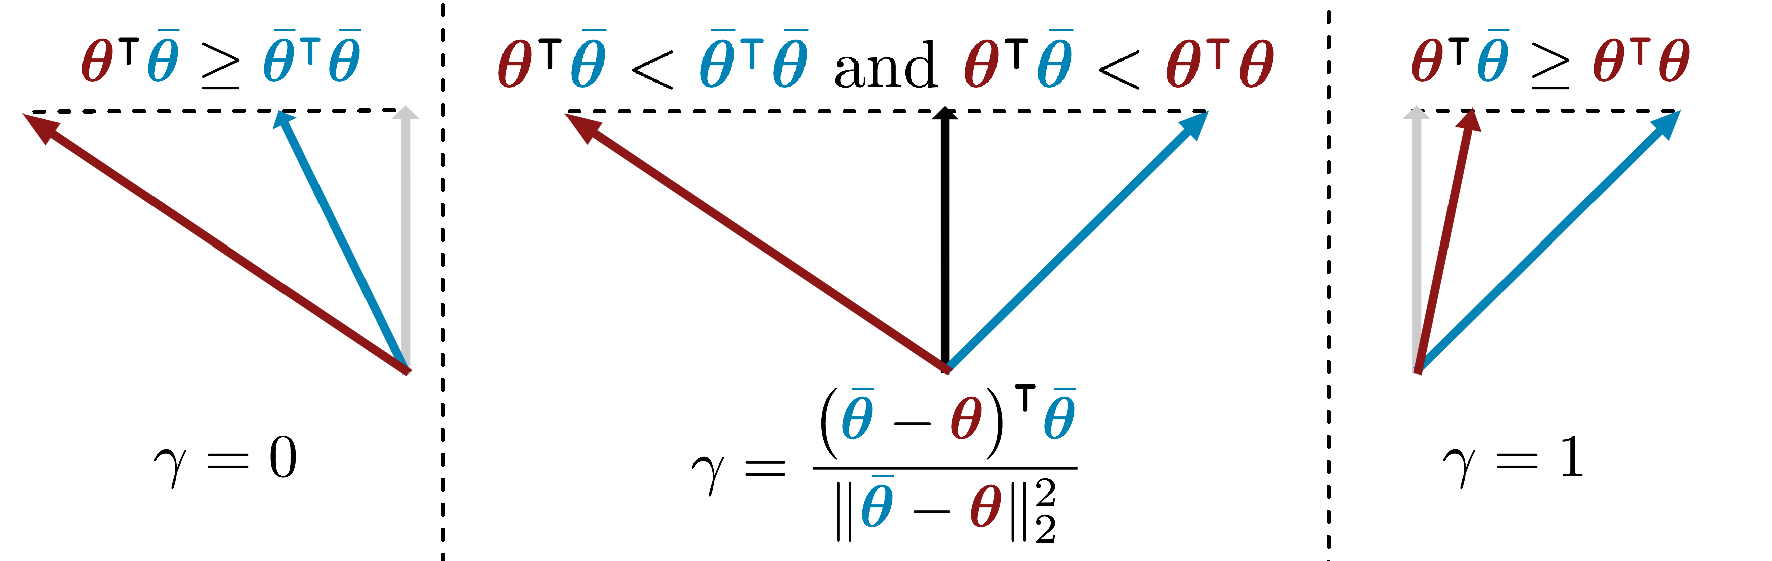
\includegraphics[width=\textwidth]{min_norm2point}
\captionof{figure}{Visualisation of the min-norm point in the convex hull of two points (\mbox{$\min_{\gamma \in [0,1]} \| \gamma \btheta + (1-\gamma) \bar{\btheta} \|_2^2$}). As the geometry suggests, the solution is either an edge case or a perpendicular vector.}
\end{minipage}
&\begin{minipage}{0.30\textwidth}
\vspace{-5mm}
\begin{algorithm}[H]\captionsetup{labelsep=newline}
\caption{ $\min_{\gamma \in [0,1]} \| \gamma \btheta + (1-\gamma) \bar{\btheta} \|_2^2$}
\label{alg:TWO_PNT}
\begin{algorithmic}[1]
\If{$\btheta^\intercal \bar{\btheta} \geq \btheta^\intercal \btheta$}
\State $\gamma = 1$
\ElsIf{$\btheta^\intercal \bar{\btheta} \geq \bar{\btheta}^\intercal \bar{\btheta}$}
\State $\gamma = 0$
\Else
\State $\gamma = \frac{(\bar{\btheta}- \btheta)^\intercal \bar{\btheta}}{\|\btheta - \bar{\btheta}\|_2^2}$
\EndIf
\end{algorithmic}
\end{algorithm}
\end{minipage}
\end{tabular}
%\vspace{-2mm}
\begin{algorithm}[H]
\caption{Update Equations for MTL}
\label{alg:mtl_mgda}
\begin{algorithmic}[1]
\For{$t=1$ {\bfseries to} $T$}
\State $\btheta^t = \btheta^t - \eta \nabla_{\btheta^{t}}  \hat{\lL}^t(\btheta^{sh},\btheta^t)$  \Comment{Gradient descent on task-specific parameters}
\EndFor
\State $\alpha^1,\ldots,\alpha^{T}$ = \textproc{FrankWolfeSolver}($\btheta$) \Comment{Solve (3) to find a common descent direction}
\State $\btheta^{sh} = \btheta^{sh} -   \eta \sum_{t=1}^T \alpha^t \nabla_{\btheta^{sh}}  \hat{\lL}^t(\btheta^{sh},\btheta^t)$ \Comment{Gradient descent on shared parameters}
\Statex
\Procedure{FrankWolfeSolver}{$\btheta$}
\State Initialize $\bm{\alpha} = (\alpha^1, \ldots, \alpha^{T}) = (\frac{1}{T}, \ldots, \frac{1}{T})$
\State Precompute $\MM$ st. $\MM_{i,j} = \big(\nabla_{\btheta^{sh}}  \hat{\lL}^i(\btheta^{sh},\btheta^i)\big)^\intercal \big(\nabla_{\btheta^{sh}}  \hat{\lL}^j(\btheta^{sh},\btheta^j)\big)$
\Repeat
\State $\hat{t} = \argmin_r \sum_t \alpha^t \MM_{rt}$
\State $\hat{\gamma} = \argmin_{\gamma}  \big( (1 - \gamma) \bm{\alpha} + \gamma \bm{e}_{\hat{t}}  \big)^\intercal \MM  \big( (1 - \gamma) \bm{\alpha} + \gamma \bm{e}_{\hat{t}}  \big)$ \Comment{Using Algorithm 1}
\State $\bm{\alpha} = (1- \hat{\gamma})\bm{\alpha} + \hat{\gamma} \bm{e}_{\hat{t}}$
\Until{$\hat{\gamma} \sim 0$ {\bfseries or} Number of Iterations Limit}
\State {\bfseries return} $\alpha^1,\ldots,\alpha^{T}$
\EndProcedure
\end{algorithmic}
\end{algorithm}
\end{minipage}


\subsection{Efficient Optimization for Encoder-Decoder Architectures}
%\subsection{Approximating the Optimization Problem}
\label{sec:approximation}

The MTL update described in Algorithm~\ref{alg:mtl_mgda} is applicable to any problem that uses optimization based on gradient descent. Our experiments also suggest that the Frank-Wolfe solver is efficient and accurate as it typically converges in a modest number of iterations with negligible effect on training time. However, the algorithm we described needs to compute $\nabla_{\btheta^{sh}} \hat{\lL}^t(\btheta^{sh},\btheta^t)$ for each task $t$, which requires a backward pass over the shared parameters for each task. Hence, the resulting gradient computation would be the forward pass followed by $T$ backward passes. Considering the fact that computation of the backward pass is typically more expensive than the forward pass, this results in linear scaling of the training time and can be prohibitive for problems with more than a few tasks.

We now propose an efficient method that optimizes an upper bound of the objective and requires only a single backward pass. We further show that optimizing this upper bound yields a Pareto optimal solution under realistic assumptions. The architectures we address conjoin a shared representation function with task-specific decision functions. This class of architectures covers most of the existing deep MTL models and can be formally defined by constraining the hypothesis class as
\begin{equation}
f^t(\xx;\btheta^{sh},\btheta^t) = (f^t(\cdot; \btheta^t) \circ g(\cdot; \btheta^{sh})) (\xx)  = f^t( g(\xx; \btheta^{sh}); \btheta^t  )
\end{equation}
where $g$ is the representation function shared by all tasks and $f^t$ are the task-specific functions that take this representation as input. If we denote the representations as \mbox{$\ZZ = \big(\zz_1,\ldots,\zz_N \big)$}, where $\zz_i = g(\xx_i;\btheta^{sh})$, we can state the following upper bound as a direct consequence of the chain rule:
\begin{equation}
  \Bigg\| \sum_{t=1}^T \alpha^t \nabla_{\btheta^{sh}}  \hat{\lL}^t(\btheta^{sh},\btheta^t) \Bigg\|_2^2  \leq    \Bigg\|\frac{\partial \ZZ}{\partial \btheta^{sh}}\Bigg\|_2^2 \Bigg\| \sum_{t=1}^T \alpha^t  \nabla_{\ZZ}  \hat{\lL}^t(\btheta^{sh},\btheta^t) \Bigg\|_2^2
  \end{equation}
where  $\left\|\frac{\partial \ZZ}{\partial \btheta^{sh}}\right\|_2$ is the matrix norm of the Jacobian of $\ZZ$ with respect to $\btheta^{sh}$. Two desirable properties of this upper bound are that (i) $\nabla_{\ZZ} \hat{\lL}^t(\btheta^{sh},\btheta^t)$ can be computed in a single backward pass for all tasks and (ii) $\left\|\frac{\partial \ZZ}{\partial \btheta^{sh}}\right\|_2^2 $ is not a function of $\alpha^1,\ldots ,\alpha^T$, hence it can be removed when it is used as an optimization objective. We replace the $\left\| \sum_{t=1}^T \alpha^t \nabla_{\btheta^{sh}}  \hat{\lL}^t(\btheta^{sh},\btheta^t) \right\|_2^2$ term with the upper bound we have just derived in order to obtain the approximate optimization problem and drop the $\left\|\frac{\partial \ZZ}{\partial \btheta^{sh}}\right\|_2^2 $ term since it does not affect the optimization. The resulting optimization problem is
\begin{equation}
\min_{\alpha^1,\ldots,\alpha^T}  \Bigg\{  \bigg\| \sum_{t=1}^T \alpha^t  \nabla_{\ZZ}  \hat{\lL}^t(\btheta^{sh},\btheta^t) \bigg\|_2^2 \bigg |  \sum_{t=1}^T \alpha^t = 1, \alpha^t \geq 0 \quad \forall t \Bigg\} \\
\eqname{(MGDA-UB)}
\label{eq:approx}
\end{equation}

We refer to this problem as MGDA-UB (Multiple Gradient Descent Algorithm -- Upper Bound). In practice, MGDA-UB corresponds to using the gradients of the task losses with respect to the representations instead of the shared parameters. We use Algorithm~\ref{alg:mtl_mgda} with only this change as the final method.

Although MGDA-UB is an approximation of the original optimization problem, we now state a theorem that shows that our method produces a Pareto optimal solution under mild assumptions. The proof is given in the supplement.

\begin{theorem}
Assume $\frac{\partial \mathbf{Z}}{\partial \mathbf{\theta}^{sh}}$ is full-rank. If $\alpha^{1,\ldots,T}$ is the solution of MGDA-UB, one of the following is true:
\begin{enumerate}[ topsep=0pt, label=\emph{(\alph*)},align=left,leftmargin=*]
\item $\sum_{t=1}^T \alpha^t \nabla_{\btheta^{sh}}  \hat{\lL}^t(\btheta^{sh},\btheta^t)=0$ and the current parameters are Pareto stationary.
\item $\sum_{t=1}^T \alpha^t \nabla_{\btheta^{sh}}  \hat{\lL}^t(\btheta^{sh},\btheta^t)$ is a descent direction that decreases all objectives.
\end{enumerate}
\label{thm}
\end{theorem}

This result follows from the fact that as long as $\frac{\partial \ZZ}{\partial \btheta^{sh}}$ is full rank, optimizing the upper bound corresponds to minimizing the norm of the convex combination of the gradients using the Mahalonobis norm defined by $\frac{\partial \ZZ}{\partial \btheta^{sh}}^\intercal \frac{\partial \ZZ}{\partial \btheta^{sh}}$. The non-singularity assumption is reasonable as singularity implies that tasks are linearly related and a trade-off is not necessary. In summary, our method provably finds a Pareto stationary point with negligible computational overhead and can be applied to any deep multi-objective problem with an encoder-decoder model.
